\documentclass{article}

\usepackage{graphicx}
\usepackage{tikz}
\usepackage{tikzsymbols}
\usetikzlibrary{calc,patterns,shapes.geometric}
\pagestyle{empty}
\usepackage[margin=0pt]{geometry}
\geometry{papersize={14in,12in}}

\def\centerarc[#1](#2)(#3:#4:#5){\draw[#1] ($(#2)+({#5*cos(#3)},{#5*sin(#3)})$) arc (#3:#4:#5);}

\begin{document}
	\begin{figure}
		\centering
		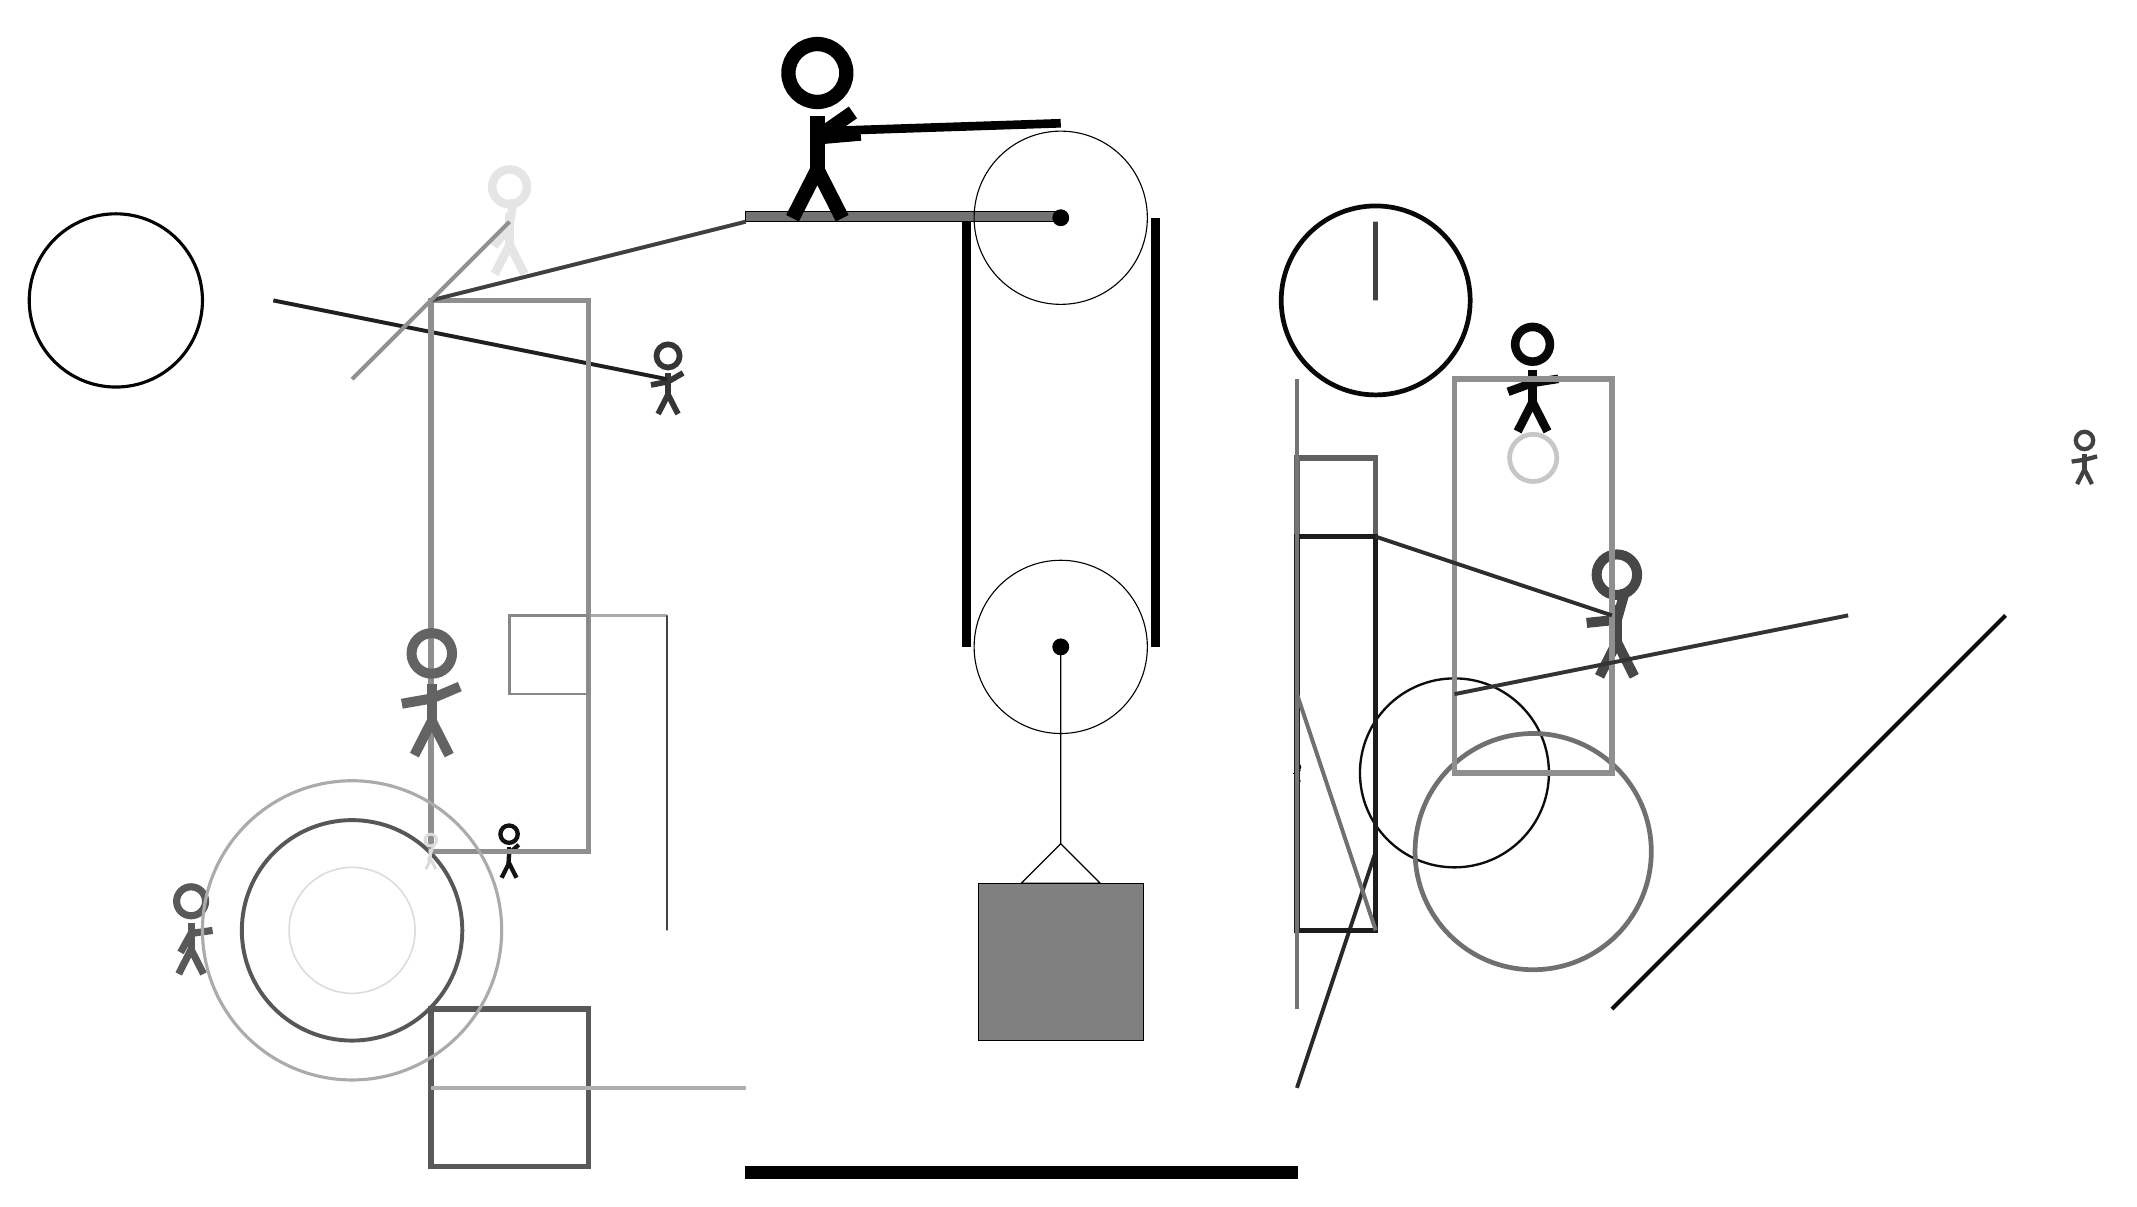
\begin{tikzpicture}
			%%%%% START %%%%%
			
			\draw[fill=black!55] (-2, 9) rectangle (2, 9.125);
			
			\draw (2, 3.6) circle (1.1);
			\draw[fill=black] (2, 3.6) circle (0.1);
			
			\draw (2, 9.05) circle (1.1);
			\draw[fill=black] (2, 9.05) circle (0.1);
			
			\draw (2, 3.6) -- (2, 1.1) -- (1.5, 0.6) -- (2.5, 0.6) -- (2, 1.1);
			\draw[fill=black!50] (0.95, 0.6) rectangle (3.05, -1.4);
			
			\draw[line width=1.1mm] (0.8, 9) -- (0.8, 3.6);
			\centerarc[line width=1.1mm](2, 3.6)(180:360:1.2000000000000002);
			\draw[line width=1.1mm](3.2, 3.6) -- (3.2, 9.05);
			\centerarc[line width=1.1mm](2, 9.05)(0:90:1.2000000000000002);
			\draw[line width=1.1mm](2, 10.25) -- (-1, 10.15);
			
			\node at (-1, 10.15) {\Strichmaxerl[10][-175][35]};
			
			\draw[line width=0.7mm, color=black!65] (-4, -3) rectangle (-6, -1);
			
			\node[line width=0.7mm, color=black!65] at (-9, 0) {\Strichmaxerl[5][61][8]};
			\draw[line width=0.3mm, color=black!33] (-3, 4) rectangle (-5, 4);
			\draw [line width=0.3mm, color=black!95](7, 2) circle (1.2);
			\node[line width=0.3mm, color=black!10] at (-5, 9) {\Strichmaxerl[6][53][81]};
			
			\draw[line width=0.7mm, color=black!62] (6, 6) rectangle (5, 0);
			
			\node[line width=0.4mm, color=black!72] at (9, 4) {\Strichmaxerl[7][6][74]};
			
			\node[line width=0.4mm, color=black!79] at (-3, 7) {\Strichmaxerl[4][11][30]};
			\draw [line width=0.5mm, color=black!66](-7, 0) circle (1.4);
			
			\draw[line width=0.7mm, color=black!74] (6, 8) rectangle (6, 9);
			
			\node[line width=0.6mm, color=black!98] at (5, 2) {\Strichmaxerl[1][0][54]};
			
			\draw [line width=0.6mm, color=black!56](8, 1) circle (1.5);
			\draw[line width=0.5mm, color=black!84](6, 1) -- (5, -2);
			\draw [line width=0.6mm, color=black!97](6, 8) circle (1.2);
			\node[line width=0.2mm, color=black!93] at (-5, 1) {\Strichmaxerl[3][87][42]};
			\draw[line width=0.5mm, color=black!88](-3, 7) -- (-8, 8);
			\node[line width=0.4mm, color=black!97] at (8, 7) {\Strichmaxerl[6][20][9]};
			
			\draw[line width=0.7mm, color=black!44] (7, 2) rectangle (9, 7);
			\draw[line width=0.7mm, color=black!44] (-4, 1) rectangle (-6, 8);
			\draw[line width=0.5mm, color=black!31](-6, -2) -- (-2, -2);
			\node[line width=0.4mm, color=black!61] at (-6, 3) {\Strichmaxerl[7][10][23]};
			\draw[line width=0.3mm, color=black!47] (-4, 3) rectangle (-5, 4);
			\draw[line width=0.7mm, color=black!89] (5, 0) rectangle (6, 5);
			\node[line width=0.5mm, color=black!14] at (-6, 1) {\Strichmaxerl[2][73][69]};
			\draw[line width=0.5mm, color=black!54](5, -1) -- (5, 7);
			
			\draw[line width=0.5mm, color=black!95](9, -1) -- (14, 4);
			\draw [line width=0.4mm, color=black!99](-10, 8) circle (1.1);
			\draw[line width=0.2mm, color=black!74] (-3, 4) rectangle (-3, 0);
			
			\draw[line width=0.5mm, color=black!82](6, 5) -- (9, 4);
			\draw [line width=0.4mm, color=black!33](-7, 0) circle (1.9);
			\draw [line width=0.6mm, color=black!22](8, 6) circle (0.3);
			
			\node[line width=0.5mm, color=black!74] at (15, 6) {\Strichmaxerl[3][8][15]};
			\draw[line width=0.5mm, color=black!75](-6, 8) -- (-2, 9);
			
			\draw[line width=0.5mm, color=black!43](-5, 9) -- (-7, 7);
			
			\draw[line width=0.5mm, color=black!56](5, 3) -- (6, 0);
			\draw [line width=0.2mm, color=black!14](-7, 0) circle (0.8);
			
			\draw[line width=0.5mm, color=black!80](7, 3) -- (12, 4);
			
			\draw[fill=black] (-2, -3) rectangle (5, -3.15);
			
			%%%%% END %%%%%
		\end{tikzpicture}
	\end{figure}	
\end{document}